%%% FIG %%%
\begin{figure}\centering
\begin{tabular}{@{}c@{}|@{}c@{}}
\includegraphics[width=.49\linewidth]{1d/cross-orient/linear-interp}&
\includegraphics[width=.49\linewidth]{1d/cross-orient/interp-ellipses}\\\hline
\includegraphics[width=.49\linewidth]{3d/plate-elong/linear-interp}&
\includegraphics[width=.49\linewidth]{3d/plate-elong/interp-ellipses}\\\hline
Linear interpolation & Quantum OT
\end{tabular}
\caption{Comparison of linear and quantum-OT interpolation (using formula~\eqref{eq-interpolating}). 
Each row shows a field of tensors (top $d=2$, bottom $d=3$) along a linear segment from $t=0$ to $t=1$ ($t$ axis is vertical).
} \label{fig:1d-interp}
\end{figure}
%%% FIG %%%